
\documentclass[xcolor=dvipsnames,aspectratio=169]{beamer}
%\documentclass[aspectratio=169]{beamer}
\usepackage{beamerthemesplit}

\setbeamersize{text margin left=0.1em}  % <- like this
\setbeamersize{text margin right=0.1em} % <- like this
\usepackage{beamerthemeshadow}
\usepackage{supertabular}
\usepackage[absolute,overlay]{textpos}
\usepackage{colortbl}
%\usepackage{slashbox}
\usetheme{Warsaw}
\useoutertheme{infolines}
\setbeamercolor {alerted text} {fg=green}
\logo{\includegraphics[height=.8cm]{Img/NIT.eps}}
\usepackage{beamerthemeshadow}
\usepackage{textcomp}
\usepackage[numbers]{natbib}
\usepackage{hhline}
\newcounter{magicrownumbers}
\newcommand\rownumber{\stepcounter{magicrownumbers}\arabic{magicrownumbers}}
\usepackage{graphicx} % Allows including images
\usepackage{booktabs} % Allows the use of \toprule, \midrule and \bottomrule in tables

\usepackage{subfig}
\usepackage{subfigure}
\usepackage{caption}
\usepackage{mathabx}
\usepackage{wrapfig}
\usepackage{tikz}
\usepackage{animate}
\usetikzlibrary{shapes.geometric, arrows}
% \usepackage{algorithmicx}
% \usepackage[linesnumbered,ruled,vlined]{algorithm2e}
\usepackage{ragged2e}
\usepackage{subfigure}

%\usepackage{slashbox}
\usecolortheme[RGB={0,0,150}]{structure}

\usepackage{mathtools}
\usepackage{algpseudocode}
\algrenewcommand\alglinenumber[1]{\tiny #1:}
\usepackage{ragged2e}
\usepackage{caption}
\usepackage[font=scriptsize,labelfont=bf]{caption}
%\usecolortheme{crane}
%\usecolortheme{name=green}
\useinnertheme{rounded}
\usepackage{graphicx,amsmath}
\usepackage{verbatim,longtable}

\usepackage{tikz}
\usetikzlibrary{trees}
\usetikzlibrary{decorations.pathmorphing}
\usetikzlibrary{decorations.markings}
\usetikzlibrary{arrows}
\usepackage{pgfplots}
\usepackage{verbatim}
\usepackage{pdflscape}
\usepackage{csquotes}
\usepackage{multirow,array, amsmath, caption, booktabs,amssymb}
%\usepackage{latexsym}
%\usepackage{longtable}
%\usepackage{lscape}
\usepackage[english]{babel}

\usepackage{amssymb,gensymb}
\usepackage{tikz}
\usepackage{adjustbox}
\usepackage{graphicx}
\usepackage{fancyhdr}
\usepackage{csquotes}

% \usepackage{cite}
%\usepackage[none]{hyphenat}
\usepackage{multicol}
%\usepackage[none]{titlesec} 
%\setcounter{secnumdepth}{4}
%\usepackage[boxed,lined,linesnumbered]{algorithm2e}
% % % % % % % % % % % % % % % % % % % % % % % %added package
\usepackage{multirow,array, amsmath, caption, booktabs,amssymb}
\usepackage{epstopdf}
\usepackage{csquotes}
\usepackage{booktabs}
\usepackage{multirow}
\usepackage{siunitx}

\usepackage{multirow}

\usepackage{caption}
\usepackage{subcaption}
\usepackage{url, lipsum}



\usepackage[utf8]{inputenc}
\usepackage{algorithm}
\usepackage{amsmath}
\usepackage[ruled,vlined]{algorithm2e}

\algrenewcommand\algorithmicrequire{\textbf{Input:}}
\algrenewcommand\algorithmicensure{\textbf{Output:}}
%\usepackage{caption}
%\usepackage[top=1.5in, bottom=1.0in, left=0.8in, right=0.8in]{geometry}
\newcolumntype{C}[1]{>{\centering\arraybackslash}m{#1}}
\newcolumntype{L}[1]{>{\raggedright\arraybackslash}m{#1}}
\newcolumntype{R}[1]{>{\raggedleft\arraybackslash}m{#1}}

\definecolor{orange}{RGB}{255,100,0}
\definecolor{deepgreen}{RGB}{0,128,0}
\definecolor{deepred}{RGB}{128,0,0}




\title[Studies On Multi - Modal Fake News Detection]{\textbf{Studies On Multi - Modal Fake News Detection}\\ \small\textit{Research Project} }
\author[Supriya Saha] {\textbf{Supriya Saha} \\\tiny (122CS0101)} 
\institute{\\ \scriptsize {\vspace{0.01cm} Supervision of}\\ \scriptsize \textbf{Prof. Shyamapada Mukherjee}\\ \vspace{0.01cm} 
\small \vspace{0.1cm}\\Department of Computer Science and Engineering\\ NIT Rourkela-769008, India}
%\date{November 3, 2012}
 \date{ \tiny  \today}
 \logo{

\includegraphics[width=1cm]{1200px-NIT_Rourkela_Colour_Logo.svg.png}}
\begin{document}
\setbeamertemplate{footline}
	{%66
		\leavevmode%
		\hbox{%
			
			\begin{beamercolorbox}[wd=.09\paperwidth,ht=2.5ex,dp=1.125ex,center]{title in head/foot}%
				\usebeamerfont{author in head/foot}\insertframenumber/\inserttotalframenumber
			\end{beamercolorbox}%
			
			\begin{beamercolorbox}[wd=.009\paperwidth,ht=2.5ex,dp=1.125ex,center]{}
			\end{beamercolorbox}%
			
			\begin{beamercolorbox}[wd=.2\paperwidth,ht=2.5ex,dp=1.125ex,center]{author in head/foot}%
				\usebeamerfont{title in head/foot}\insertshortauthor\hspace{.3cm}
			\end{beamercolorbox}%
			
			\begin{beamercolorbox}[wd=.005\paperwidth,ht=2.5ex,dp=1.125ex,center]{}
			\end{beamercolorbox}%
			
			\begin{beamercolorbox}[wd=.7\paperwidth,ht=2.5ex,dp=1.125ex,center]{title in head/foot}%
				\usebeamerfont{author in head/foot}\hspace{.3cm}\insertshorttitle
			\end{beamercolorbox}%
		}%
		\vskip0pt%
	}
	

\tikzset{
	photon/.style={decorate, decoration={snake}, draw=red},
	VectorDAM/.style={draw=black, postaction={decorate},
		decoration={markings,mark=at position .55 with {\arrow[draw=black]{>}}},
		decoration={markings,mark=at position .05 with {\arrow[draw=black]{*}} },
		decoration={markings,mark=at position .95 with {\arrow[draw=black]{*}} } },
	VectorAM/.style={draw=black, postaction={decorate},
		decoration={markings,mark=at position .55 with {\arrow[draw=black]{>}}} },
	gluon/.style={decorate, draw=magenta, decoration={coil,amplitude=4pt, segment length=5pt}} 
}
 \frame{\titlepage}
%\frame{\frametitle{\begin{footnotesize}Introductions\end{footnotesize}}
%\begin{scriptsize}\tableofcontents\end{scriptsize}









\frame{\frametitle{Outline}
%\begin{scriptsize}

\tableofcontents%\end{scriptsize}
}
\setbeamertemplate{caption}[numbered]


%%%%%%%%%%%%%%%%%%%%%%%%%%%%%%%%%%%%%%%%%%%%%%%%%%%%%%%%%%%%%%%%%%%%%%%%







%%%%%%%%%%%%%%%%%%%%%%%%%%%%%%%%%%%%%%%%%%%%%%%%%%%%%%%%%%%%%%%%%%%%%%%%
\section{Introduction}
\begin{frame}{Introduction}

	\begin{itemize}
		\item Misinformation spreads quickly on social media using both text and images which creates a multimodal detection challenge. \\
        
        \item Traditional models treat text and images separately or fuse them weakly, leading to poor semantic alignment and limited interpretability.\\
        
        \item SpotFake uses BERT (text) + VGG19 (image) with simple fusion but this limits its ability to handle complex, real-world misinformation. \\
        
        \item Recent advances improve this by:
        \begin{itemize}
            \item Contrastive Learning (CLIP-style): Aligns text–image embeddings for stronger cross-modal understanding.
            \item Cross-Modal Attention: Focuses on the most informative tokens or regions.
            \item Explainability (Grad-CAM, SHAP): Displays decision reasoning for transparency.
        \end{itemize}
	\end{itemize}
\end{frame}






%%%%%%%%%%%%%%%%%%%%%%%%%%%%%%%%%%%%%%%%%%%%%%%%%%%%%%%%%%%%%%%%%%%%%%%%%%%





%%%%%%%%%%%%%%%%%%%%%%%%%%%%%%%%%%%%%%%%%%%%%%%%%%%%%%%%%%%%%%%%%%%%%%%%%%%%%%%%



%%%%%%%%%%%%%%%%%%%%%%%%%%%%%%%%%%%%%%%%%%%%%%%%%%%%%%%%%%%%%%%%%


%%%%%%%%%%%%%%%%%%%%%%%%%%%%%%%%%%%%%%%%%%%%%%%%%%%%%%%%%%%%%%%%%%%%%%%%%
		
%%%%%%%%%%%%%%%%%%%%%%%%%%%%%%%%%%%%%%%%%%%%%%%%%%%%%%%%%%%%%%%%%%%%%%%%%%
\section{Literature Review}
\begin{frame}{Literature Review}
    \begin{table}[]
    \caption{Recent Literature on Multi - Modal Fake News Detection.}
    \centering
    {\tiny %
    \begin{tabular}{|p{2.0cm}|p{1.0cm}|p{1.5cm}|p{2.5cm}|p{2.5cm}|p{1.5cm}|p{1.0cm}|}
    \hline
    \textbf{Reference} & \textbf{Model} & \textbf{Method} & \textbf{Merits} & \textbf{Drawbacks} & \textbf{Dataset} & \textbf{Accuracy Measure} \\ \hline
    
    Abbas Khosravi et al. (2011), IEEE Transactions on Neural Networks \cite{12} & Neural Networks & LUBE (Lower-Upper Bound Estimation) & Produces reliable prediction intervals without assuming noise distribution. Applicable to various forecasting problems. & Tuning of custom loss functions is complex. Training instability may occur. & Benchmark time series datasets & PICP, PINAW \\ \hline
    
    Cameron Cornell et al. (2024), Int. Journal of Forecasting \cite{2} & Neural Networks & Probabilistic Forecasting for Electricity Prices & Adapts well to market volatility, integrates market mechanisms in forecasting. & Model sensitivity to sudden price spikes and data availability issues. & Australian National Electricity Market (NEM) & CRPS, RMSE, PICP \\ \hline
    
    Yan Xu et al. (2024), Computers and Industrial Engineering \cite{9} & Quantile Regression & Quantile Combination Forecasting & Combines multiple quantile forecasts to improve robustness and accuracy. & Complexity in selecting and weighting contributing models. & Electricity price datasets & PICP, Quantile Loss \\ \hline
    
    Sourav Kumar Purohit and S. Panigrahi (2024), Information Sciences \cite{1} & Hybrid (Statistical + DL) & Probabilistic Forecasting using Optimized DL & Integrates classical and deep models for improved oil price forecasting. & High computational demand; interpretability challenges. & Crude oil market datasets & RMSE, MAE, PICP \\ \hline
    
    H{\"a}rdle et al. (2003), Int. Statistical Review \cite{Bootstrap} & Statistical & Bootstrap Methods & Resampling preserves temporal dependence; useful for interval estimation in small samples. & Assumes stationarity; performance degrades with non-stationary or highly volatile data. & Synthetic and economic time series & Coverage, Bias, Variance \\ \hline
    
    \end{tabular}
    }
    \label{tab:my_label}
\end{table}


\end{frame}

\begin{frame}{Literature Survey(Cont.)}
    \begin{itemize}
        \item According to literature review these were the most frequently used probabilistic forecasting methods:

        \begin{figure}
            \centering
            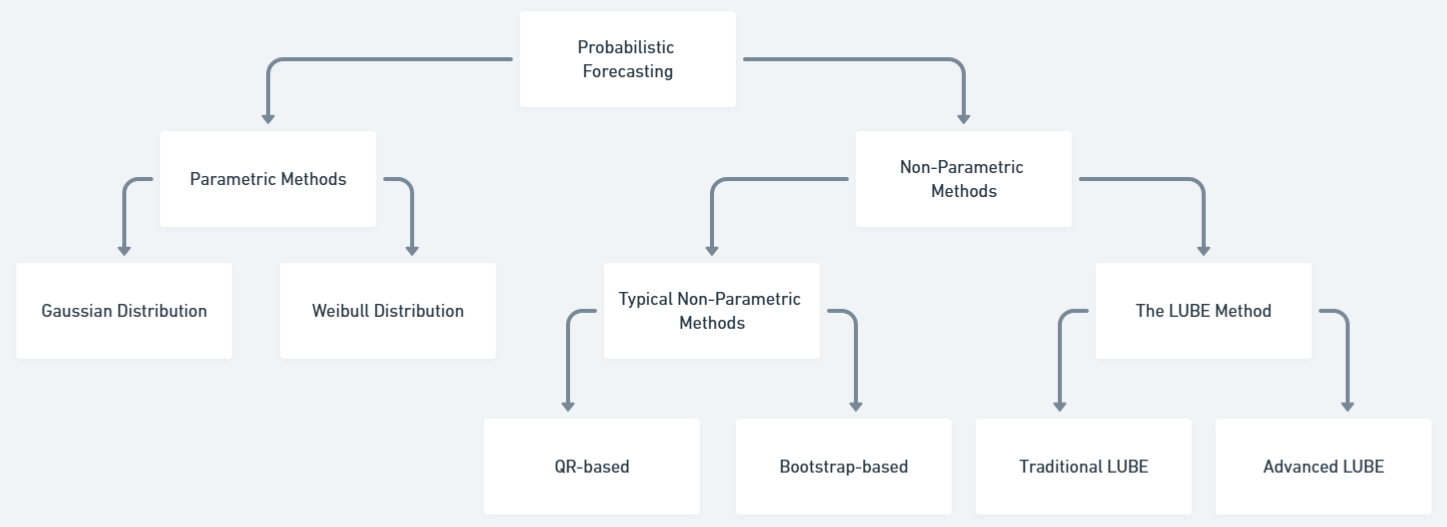
\includegraphics[width=0.8\linewidth]{Classification Of Probabilistic Methods.jpg}
            \caption{Classification of Traditional Probabilistic Forecasting Methods.}
            \label{fig:enter-label}
        \end{figure}
    \end{itemize}
    
\end{frame}

\begin{frame}{Key Insights from Recent Literature}
    \begin{itemize}
        \item Handling uncertainty through interval predictions has become a standard for time series forecasting tasks.
        \item Combining statistical and deep learning techniques enhances accuracy and flexibility in forecasting.
        \item Metrics like PICP (Prediction Interval Coverage Probability), PINAW (Prediction Interval Normalized Average Width), ACE (Absolute Coverage Error) and AWE (Average Width Error) are widely adopted for comprehensive performance assessment.
    \end{itemize}
\end{frame}


\begin{frame}{Key Insights from Recent Literature (Cont.)}
    \begin{itemize}
        \item \textbf{Research Gap:} No comprehensive studies comparing the parametric and non-parametric methods and their performance on a variety of datasets under different confidence levels are conducted. Also, there is a lack of hybrid methods.

        \item \textbf{Contribution: } Examined the performance of six traditional probabilistic forecasting methods across a variety of datasets using different evaluation metrics to assess their performance. Also developed two hybrid methods that out-performs the traditional methods.
    \end{itemize}
\end{frame}



\section{Objectives}


\begin{frame}{Objectives}
		
        \begin{itemize}
		
        \item Develop a BERT + ResNet50 multimodal model (compare with VGG19).\\

        \item Apply CLIP-style contrastive pre-training for text–image alignment.\\

        \item Introduce cross-modal attention for selective, context-aware fusion.\\

        \item Integrate explainability tools — Grad-CAM, SHAP and attention heatmaps for interpretable predictions.
		
		\end{itemize}
    
\end{frame}
%%%%%%%%%%%%%%%%%%%%%%%%%%%%%%%%%%%%%%%%%%%%%%%%%%%%%%%%%%%%%%%%%%%%%%%%%%%

%%%%%%%%%%%%%%%%%%%%%%%%%%%%%%%%%%%%%%%%%%%%%%%%%%%%%%%%%%%%%%%%%%%%%%%%%


	
%%%%%%%%%%%%%%%%%%%%%%%%%%%%%%%%%%%%%%%%%%%%%%%%%%%%%%%%%%%%%%%%%%%%%%%%%%%%%

%%%%%%%%%%%%%%%%%%%%%%%%%%%%%%%%%%%%%%%%%%%%%%%%%%%%%%%%
\section{Dataset Overview}
\begin{frame}{Dataset Overview}

\begin{table}[!ht]
    \caption{Summary of Datasets Used.}
    \centering
    \begin{tabular}{|p{5cm}|c|}
        \hline
        \textbf{Dataset Name} & \textbf{Length of Dataset} \\
        \hline
        \multicolumn{2}{|c|}{\textbf{Nifty50 Dataset (2000--2021)}} \\
        \hline
        Adani Ports & 3322 \\
        Asian Paints & 5306 \\
        Axis Bank & 5306 \\
        \hline
        Web Traffic & 550 \\
        Electricity Consumption & 1858 \\
        \hline
    \end{tabular}
    \label{tab:dataset_summary}
\end{table}

\end{frame}



%%%%%%%%%%%%%%%%%%%%%%%%%%%%%%%%%%%%%%%%%%%%%%%%%%%%%%%%%%%%%%%%%%%%%%%%
\section{Evaluation Metrics}
\begin{frame}{Evaluation Metrics}
\begin{itemize}
    \item \textbf{PICP (Prediction Interval Coverage Probability):} Proportion of true values within prediction intervals.
    \item \textbf{PINAW (Prediction Interval Normalized Average Width):} Width of intervals (normalized).
    \item \textbf{ACE (Absolute Coverage Error):} Absolute difference between the actual coverage (PICP) and the desired confidence level.
    \item \textbf{AWE (Average Width Error:)} Average deviation of the widths of the prediction intervals from an expected or desired width.
\end{itemize}
    
\end{frame}






%%%%%%%%%%%%%%%%%%%%%%%%%%%%%%%%%%%%%%%%%%%%%%%%%%%%%%%%%%%%%%%%%%%%%%%%%%%%%%%%%%%%%%%%%%%%
\section{Methodology}
\begin{frame}{Methodology}
\begin{figure}
    \centering
    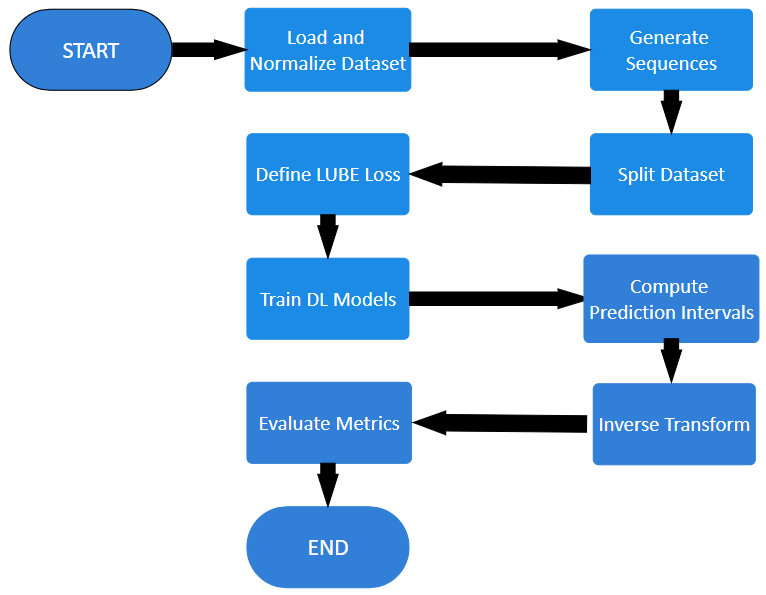
\includegraphics[width=0.5\linewidth]{TLUBE.png}
    \caption{Traditional LUBE Method Flowchart.}
    \label{fig:enter-label}
\end{figure}
\end{frame}

\begin{frame}{Methodology (Cont.)}
        \begin{algorithm}[H]
        \tiny
        \SetAlgoNlRelativeSize{0}
        \SetAlgoCaptionSeparator{:}
        
        \KwIn{Time series dataset $D$}
        \KwOut{Predicted intervals $[LB, UB]$, PICP, PINAW, ACE, AWE}
        
        \textbf{Step 1: Data Preprocessing}\\
        Normalize $D$ using MinMaxScaler\\
        Generate input-output pairs with window size $w$\\
        Split into train, validation and test sets
        
        \textbf{Step 2: Define LUBE Loss}\\
        \ForEach{$c \in \{0.9, 0.8, 0.7, 0.6\}$}{
            $q = 1 - c$\\
            Compute $LB$, $UB$\\
            Compute $\text{Loss}_{\text{lower}}$ and $\text{Loss}_{\text{upper}}$\\
            Compute \text{PICP}\\
            Compute $\text{Loss}_{\text{LUBE}}$
        }
        
        \textbf{Step 3: Model Training}
        \ForEach{$M \in \{$LSTM, CNN, GRU, BiLSTM$\}$}{
            Define model architecture\\
            Compile with LUBE loss\\
            Train on $(X_{\text{train}}, y_{\text{train}})$ for $e$ epochs\\
            Validate on $(X_{\text{val}}, y_{\text{val}})$\\
            Save $LB, UB$ for test data
        }
        
        \textbf{Step 4: Evaluation Metrics} Compute the PINAW, ACE and AWE of the computed prediction intervals.
        
        \textbf{Step 5: Aggregate Results} Compute mean of metrics for all models
        
        \caption{Traditional LUBE Method.}
        \end{algorithm}

    
\end{frame}

\begin{frame}{Methodology (Cont.)}
\begin{figure}
    \centering
    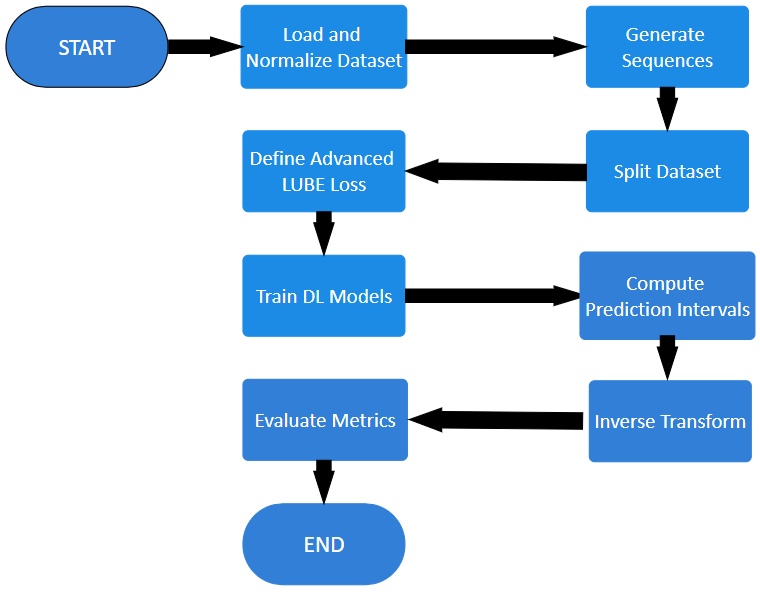
\includegraphics[width=0.5\linewidth]{ALUBE.png}
    \caption{Advanced LUBE Method Flowchart.}
    \label{fig:enter-label}
\end{figure}
\end{frame}

\begin{frame}{Methodology (Cont.)}
        \begin{algorithm}[H]
        \tiny
        \SetAlgoNlRelativeSize{0}
        \SetAlgoCaptionSeparator{:}
        
        \KwIn{Time series dataset $D$}
        \KwOut{Predicted intervals $[LB, UB]$, PICP, PINAW, ACE, AWE}
    
        \textbf{Step 1: Data Preprocessing}\\
        Normalize $D$ using MinMaxScaler\\
        Generate input-output pairs with window size $w$\\
        Split into train, validation and test sets
    
        \textbf{Step 2: Define Advanced LUBE Loss}\\
        \ForEach{$c \in \{0.9, 0.8, 0.7, 0.6\}$}{
            $q = 1 - c$\\
            Compute $LB$, $UB$\\
            Compute $\text{Loss}_{\text{lower}}$ and $\text{Loss}_{\text{upper}}$\\
            Compute PICP and PINAW \\
            Compute $\text{Loss}_{\text{LUBE}}$
        }
    
        \textbf{Step 3: Model Training}\\
        \ForEach{$M \in \{$LSTM, CNN, GRU, BiLSTM$\}$}{
            Define model architecture\\
            Compile with Advanced LUBE loss\\
            Train on $(X_{\text{train}}, y_{\text{train}})$ for $e$ epochs\\
            Validate on $(X_{\text{val}}, y_{\text{val}})$\\
            Save $LB, UB$ for test data
        }
    
        \textbf{Step 4: Evaluation Metrics}
        Compute the ACE and AWE of the computed prediction intervals.
    
        \textbf{Step 5: Aggregate Results}
        Compute mean of metrics for all models and confidence levels
        
        \caption{Advanced LUBE Method.}
        \end{algorithm}
\end{frame}

\begin{frame}{Methodology (Cont.)}
\begin{figure}
    \centering
    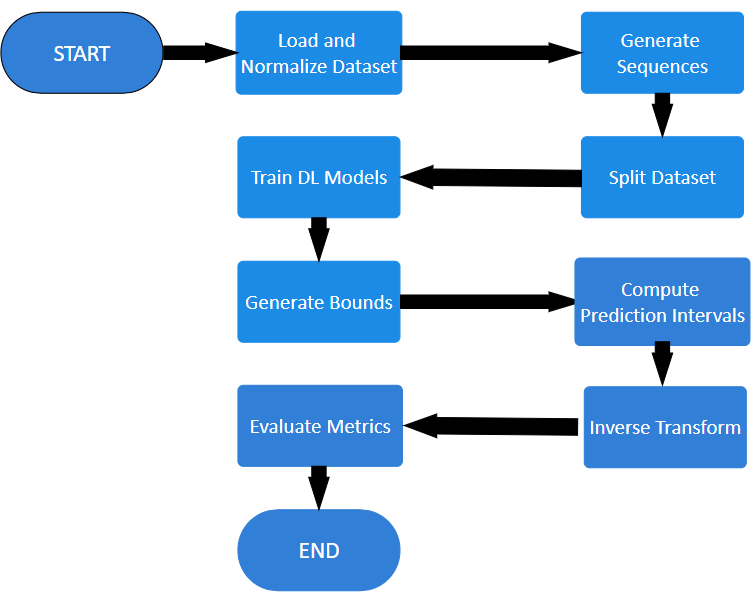
\includegraphics[width=0.5\linewidth]{QR_based.png}
    \caption{Quantile Regression based Method Flowchart.}
    \label{fig:enter-label}
\end{figure}
\end{frame}

\begin{frame}{Methodology (Cont.)}
        \begin{algorithm}[H]
        \tiny
        \SetAlgoNlRelativeSize{0}
        \SetAlgoCaptionSeparator{:}

        \KwIn{Time series dataset $D$}
        \KwOut{Predicted intervals $[LB, UB]$, PICP, PINAW, ACE, AWE}
    
        \textbf{Step 1: Data Preprocessing}\\
        Normalize $D$ using MinMaxScaler\\
        Generate input-output pairs with window size $w$\\
        Split into train, validation and test sets
    
        \textbf{Step 2: Define QR Loss Function}\\
        \ForEach{$c \in \{0.9, 0.8, 0.7, 0.6\}$}{
            Compute $q_{\text{lower}}$ and $q_{\text{upper}}$\\
            Compute $LB$, $UB$\\
            Compute $Loss_{\text{lower}}$ and $Loss_{\text{upper}}$\\
            Compute PICP and PINAW \\
            Compute $Loss_{\text{QR}}$
        }
    
        \textbf{Step 3: Model Training}\\
        \ForEach{$M \in \{$LSTM, CNN, GRU, BiLSTM$\}$}{
            Define model architecture\\
            Compile with QR-based loss\\
            Train on $(X_{\text{train}}, y_{\text{train}})$ for $e$ epochs\\
            Validate on $(X_{\text{val}}, y_{\text{val}})$\\
            Save $LB, UB$ for test data
        }
    
        \textbf{Step 4: Evaluation Metrics}
        Compute ACE and AWE of the computed prediction intervals.
    
        \textbf{Step 5: Aggregate Results}
        Compute mean of metrics for all models and confidence levels
    
        \caption{Quantile Regression (QR) based Method.}
        \end{algorithm}
\end{frame}

\begin{frame}{Methodology (Cont.)}
\begin{figure}
    \centering
    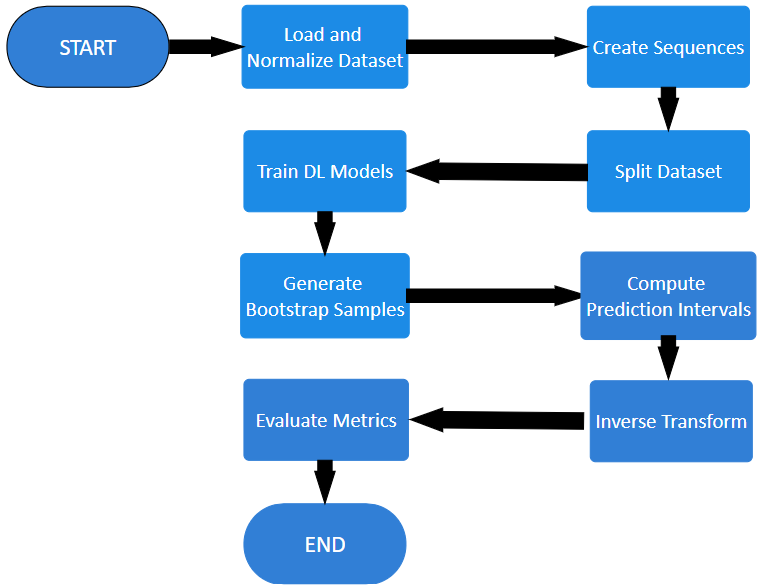
\includegraphics[width=0.5\linewidth]{Bootstrap.png}
    \caption{Bootstrap based Method Flowchart.}
    \label{fig:enter-label}
\end{figure}
\end{frame}

\begin{frame}{Methodology (Cont.)}
\begin{algorithm}[H]
\tiny
\SetAlgoNlRelativeSize{0}
\SetAlgoCaptionSeparator{:}

\KwIn{Time series dataset $D$}
\KwOut{Predicted intervals $[LB, UB]$, PICP, PINAW, ACE, AWE}

\textbf{Step 1: Data Preprocessing}\\
Normalize $D$ using MinMaxScaler\\
Generate input-output pairs with window size $w$\\
Split into train, validation and test sets

\textbf{Step 2: Model Training}\\
\ForEach{model $M \in \{$LSTM, CNN, GRU, BiLSTM$\}$}{
    Train $M$ on $(X_{\text{train}}, y_{\text{train}})$ for $e$ epochs using MSE loss
}

\textbf{Step 3: Bootstrap Prediction Intervals}\\
\ForEach{confidence level $c \in \{0.9, 0.8, 0.7, 0.6\}$}{
    \ForEach{trained model $M$}{
        Generate $B$ bootstrap samples from $X_{\text{test}}$\\
        Predict $y_{\text{pred}}$ on each sample using $M$\\
        For each $y^i_{\text{test}}$, compute $LB_i$ and $UB_i$ as empirical quantiles at $q_{\text{lower}}$ and $q_{\text{upper}}$
    }
}

\textbf{Step 4: Evaluation Metrics}
Compute PICP, PINAW, ACE and AWE for each model and confidence level

\textbf{Step 5: Aggregate Results}
Compute mean of all metrics across all runs

\caption{Bootstrap based Method.}
\end{algorithm}

\end{frame}

\begin{frame}{Methodology (Cont.)}
\begin{figure}
    \centering
    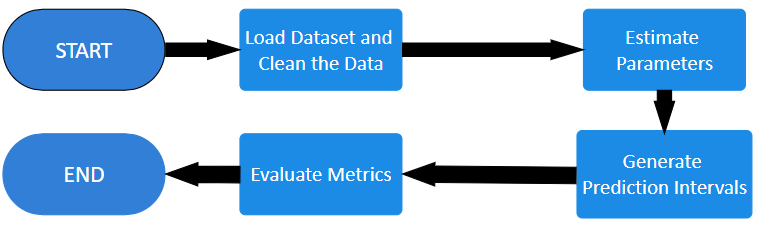
\includegraphics[width=0.6\linewidth]{GD.png}
    \caption{Gaussian Distribution based Method Flowchart.}
    \label{fig:enter-label}
\end{figure}
\end{frame}

\begin{frame}{Methodology (Cont.)}
        \begin{algorithm}[H]
        \tiny
        \SetAlgoNlRelativeSize{0}
        \SetAlgoCaptionSeparator{:}
        \KwIn{Time series dataset $D$ with target variable $y$}
        \KwOut{Predicted intervals $[LB, UB]$, PICP, PINAW, ACE, AWE}
    
        \textbf{Step 1: Data Preprocessing}\\
        Remove missing values to obtain cleaned target $y$
    
        \textbf{Step 2: Define Confidence Levels}\\
        $C = \{0.9, 0.8, 0.7, 0.6\}$
    
        \textbf{Step 3: Estimate Distribution Parameters}\\
        Compute mean $\mu$ and standard deviation $\sigma$ of $y$
    
        \textbf{Step 4: Generate Prediction Intervals}\\
        \ForEach{$c \in C$}{
            Compute $z_c$ \\
            Compute LB and UB
        }
    
        \textbf{Step 5: Evaluation Metrics} Compute the PICP, PINAW, ACE and AWE of the computed prediction intervals.\\
        \textbf{Step 6: Aggregate Results} Compute mean of all metrics across all runs 
        \caption{Gaussian Distribution based Method.}
        \end{algorithm}

\end{frame}

\begin{frame}{Methodology (Cont.)}
\begin{figure}
    \centering
    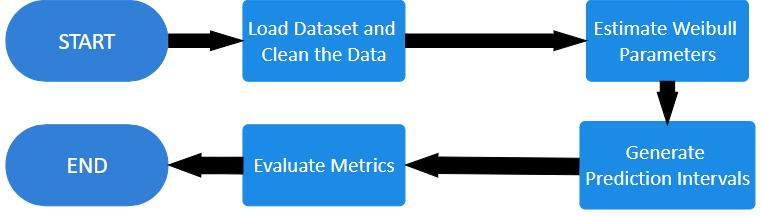
\includegraphics[width=0.6\linewidth]{WD.png}
    \caption{Weibull Distribution based Method Flowchart.}
    \label{fig:enter-label}
\end{figure}
\end{frame}

\begin{frame}{Methodology (Cont.)}
        \begin{algorithm}[H]
        \tiny
        \SetAlgoNlRelativeSize{0}
        \SetAlgoCaptionSeparator{:}

        \KwIn{Time series dataset $D$ with target variable $y$}
        \KwOut{Predicted intervals $[LB, UB]$, PICP, PINAW, ACE, AWE}
    
        \textbf{Step 1: Data Preprocessing}\\
        Remove missing values to obtain cleaned target $y$
    
        \textbf{Step 2: Define Confidence Levels}\\
        $C = \{0.9, 0.8, 0.7, 0.6\}$
    
        \textbf{Step 3: Estimate Weibull Parameters}\\
        Fit Weibull distribution to $y$ using Maximum Likelihood Estimation (MLE)\\
        Obtain shape $\kappa$, scale $\lambda$, and location $\theta$ (fixed to 0)
    
        \textbf{Step 4: Generate Prediction Intervals}\\
        \ForEach{$c \in C$}{
            Compute $\alpha$\\
            Compute LB and UB
        }
    
        \textbf{Step 5: Evaluation Metrics} Compute the PICP, PINAW, ACE and AWE of the computed prediction intervals.\\
        \textbf{Step 6: Aggregate Results} Compute mean of all metrics across all runs 
        \caption{Weibull Distribution based Method.}
        \end{algorithm}

\end{frame}

\begin{frame}{Methodology (Cont.)}
\begin{figure}
    \centering
    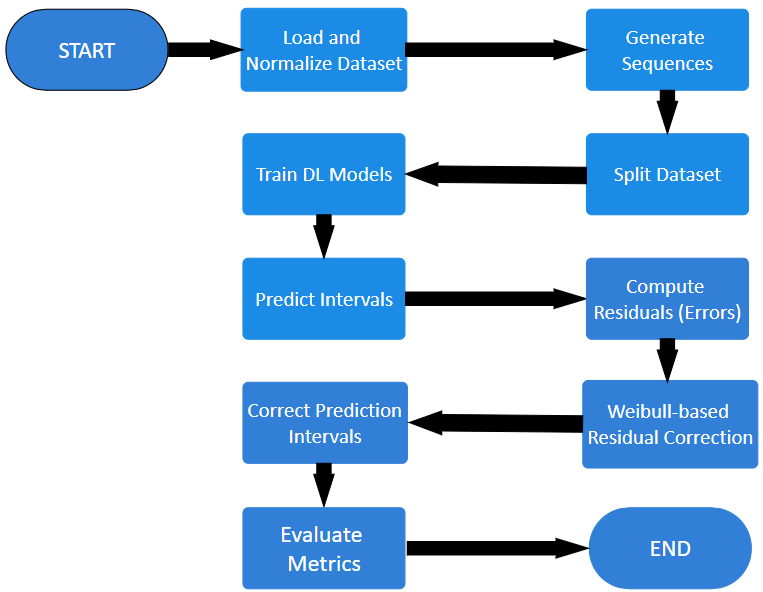
\includegraphics[width=0.5\linewidth]{LUBE_Weibull.png}
    \caption{LUBE-Weibull based Hybrid Method Flowchart.}
    \label{fig:enter-label}
\end{figure}
\end{frame}

\begin{frame}{Methodology (Cont.)}
    \begin{algorithm}[H]
        \tiny
        \SetAlgoNlRelativeSize{-1}
        \SetAlgoCaptionSeparator{:}

        \KwIn{Time series dataset $D$}
        \KwOut{Predicted intervals $[LB, UB]$, PICP, PINAW, ACE, AWE}
        
        \textbf{Step 1: Data Preprocessing}\\
        Normalize $D$ using MinMaxScaler\\
        Generate input-output pairs with window size $w$, 
        Split into train, validation, and test sets
        
        \textbf{Step 2: Define Advanced LUBE Loss}\\
        \ForEach{$c \in \{0.9, 0.8, 0.7, 0.6\}$}{
            $q = 1 - c$\\
            Compute $LB$, $UB$, Compute $\text{Loss}_{\text{lower}}$ and $\text{Loss}_{\text{upper}}$\\
            Compute PICP and PINAW\\
            Compute $\text{Loss}_{\text{LUBE}}$
        }
        
        \textbf{Step 3: Model Training}\\
        \ForEach{$M \in \{$LSTM, CNN, GRU, BiLSTM$\}$}{
            Define model architecture, 
            Compile with Advanced LUBE loss\\
            Train on $(X_{\text{train}}, y_{\text{train}})$ for $e$ epochs\\
            Validate on $(X_{\text{val}}, y_{\text{val}})$\\
            Predict $LB, UB$ for test data
        }
        
        \textbf{Step 4: Weibull Distribution Fitting on Residuals}\\
        Compute residuals $r$\\
        Estimate Weibull parameters $(\hat{k}, \hat{\lambda})$ using MLE
        
        \textbf{Step 5: Adjust Prediction Intervals Using Weibull Correction}\\
        \ForEach{$c \in \{0.9, 0.8, 0.7, 0.6\}$}{
            Compute Weibull-based correction factor $\delta_c$
        }
        
        \textbf{Step 6: Evaluation Metrics} Compute PICP, PINAW, ACE and AWE of the computed prediction intervals.
        
        \textbf{Step 7: Aggregate Results} Compute mean of all metrics across all runs
        
        \caption{Proposed Hybrid LUBE-Weibull Method.}
    \end{algorithm}
\end{frame}

\begin{frame}{Methodology (Cont.)}
\begin{figure}
    \centering
    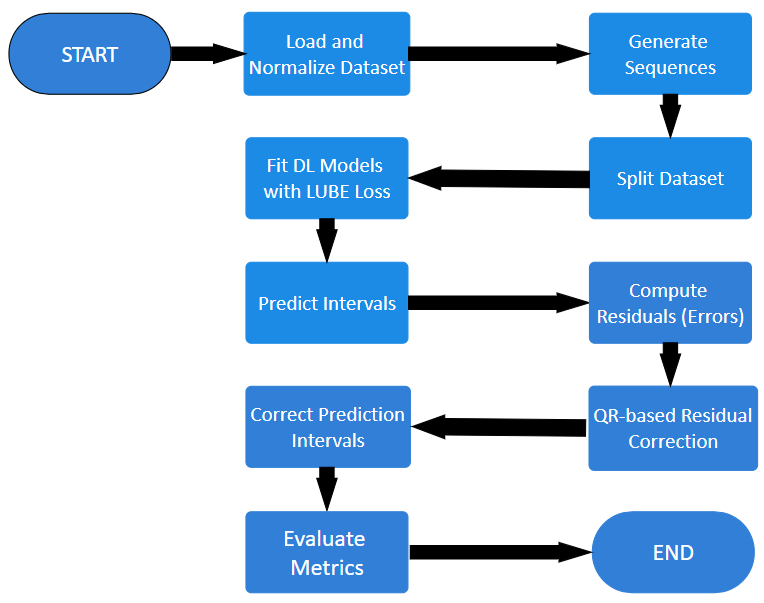
\includegraphics[width=0.5\linewidth]{LUBE_QR.png}
    \caption{LUBE-QR based Hybrid Method Flowchart.}
    \label{fig:enter-label}
\end{figure}
\end{frame}

\begin{frame}{Methodology (Cont.)}
    \begin{algorithm}[H]
        \tiny
        \SetAlgoNlRelativeSize{-1}
        \SetAlgoCaptionSeparator{:}

        \KwIn{Time series dataset $D$}
        \KwOut{Predicted intervals $[LB', UB']$, PICP, PINAW, ACE, AWE}
        
        \textbf{Step 1: Data Preprocessing}\\
        Normalize $D$ using MinMaxScaler\\
        Generate input-output pairs with window size $w$,
        Split into train, validation, and test sets
        
        \textbf{Step 2: Define Advanced LUBE Loss}\\
        \ForEach{$c \in \{0.9, 0.8, 0.7, 0.6\}$}{
            $q = 1 - c$\\
            Compute $LB$, $UB$, 
            Compute $\text{Loss}_{\text{lower}}$ and $\text{Loss}_{\text{upper}}$\\
            Compute PICP and PINAW, 
            Compute $\text{Loss}_{\text{LUBE}}$.
        }
        
        \textbf{Step 3: Model Training}\\
        \ForEach{$M \in \{$LSTM, CNN, GRU, BiLSTM$\}$}{
            Define model architecture, 
            Compile with Advanced LUBE loss\\
            Train on $(X_{\text{train}}, y_{\text{train}})$ for $e$ epochs, 
            Validate on $(X_{\text{val}}, y_{\text{val}})$\\
            Predict LUBE bounds $LB, UB$ on test data, 
            Compute midpoint $\hat{y}$
        }
        
        \textbf{Step 4: Fit Quantile Regression on Residuals}\\
        Compute residuals\\
        \ForEach{$c \in \{0.9, 0.8, 0.7, 0.6\}$}{
            Train Quantile Regression models to estimate 
            Lower quantile and Upper quantile and
            Predict residual quantiles $\hat{r}_{\text{lower}}, \hat{r}_{\text{upper}}$
        }
        
        \textbf{Step 5: Adjust Prediction Intervals Using QR Correction}\\
        \ForEach{$c \in \{0.9, 0.8, 0.7, 0.6\}$}{
            $LB' = \hat{y} + \hat{r}_{\text{lower}}$, $UB' = \hat{y} + \hat{r}_{\text{upper}}$
        }
    
        \textbf{Step 6: Evaluation Metrics} Compute the PICP, PINAW, ACE and AWE of the computed prediction intervals.
    
        
        \textbf{Step 7: Aggregate Results} Compute mean of all metrics across all runs\\
        
        \caption{Proposed Hybrid LUBE–QR Method.}
    \end{algorithm}

\end{frame}
%%%%%%%%%%%%%%%%%%%%%%%%%%%%%%%%%%%%%
\section{Experimental Setup}
\begin{frame}{Experimental Setup}
\begin{itemize}
    \item All the experiments are conducted on Acer Nitro V Laptop containing i7 12th Gen Processor, 32 GB DDR4 RAM and RTX 3070 Ti Graphics Card. 
    \item Jupyter Notebook was used to run the simulations using the Python programming language (Python 3.11.5) within the Anaconda Navigator on Windows 11 OS version 23H2.
\end{itemize}
    
\end{frame}



%%%%%%%%%%%%%%%%%%%%%%%%%%%%%%%%%%%%%%%%%%%%%%%%%%%
\section{Simulation Results}
\begin{frame}{Simulation Results}
\begin{table*}
\centering
\captionof{table}{Performance Comparison of Non-Parametric Methods on PICP Metric.}
\renewcommand{\arraystretch}{0.6}
\tiny
\resizebox{\textwidth}{!}{%
\begin{tabular}{|l|l|c|c|c|c|}
\hline
\textbf{Dataset} & \textbf{Method Used} & \multicolumn{4}{c|}{\textbf{Confidence Levels}} \\ \cline{3-6}
 & & \textbf{0.6} & \textbf{0.7} & \textbf{0.8} & \textbf{0.9} \\ \hline

Adani Ports & Traditional LUBE with LSTM & 100 & 100 & 100 & 100 \\ \cline{2-6}
 & Advanced LUBE with CNN & 100 & 100 & 100 & 100 \\ \cline{2-6}
 & QR-based with CNN & 79.07 & 86.96 & 86.74 & 95.73 \\ \cline{2-6}
 & Bootstrap-based with GRU & 58.95 & 68.43 & 78.29 & 88.05 \\ \hline

Asian Paints & Traditional LUBE with LSTM & 100 & 100 & 100 & 100 \\ \cline{2-6}
 & Advanced LUBE with CNN & 100 & 100 & 100 & 100 \\ \cline{2-6}
 & QR-based with CNN & 81.00 & 95.28 & 94.19 & 98.68 \\ \cline{2-6}
 & Bootstrap-based with GRU & 58.70 & 69.01 & 78.91 & 88.70 \\ \hline

Electricity Consumption & Traditional LUBE with LSTM & 100 & 100 & 100 & 100 \\ \cline{2-6}
 & Advanced LUBE with CNN & 99.68 & 99.67 & 99.67 & 99.69 \\ \cline{2-6}
 & QR-based with CNN & 56.94 & 73.78 & 82.73 & 87.52 \\ \cline{2-6}
 & Bootstrap-based with GRU & 19.50 & 28.20 & 31.76 & 41.40 \\ \hline

Web Traffic & Traditional LUBE with LSTM & 100 & 100 & 100 & 100 \\ \cline{2-6}
 & Advanced LUBE with CNN & 99.96 & 99.92 & 99.41 & 99.19 \\ \cline{2-6}
 & QR-based with CNN & 15.12 & 18.41 & 24.39 & 19.51 \\ \cline{2-6}
 & Bootstrap-based with GRU & 20.12 & 26.82 & 35.24 & 42.31 \\ \hline

\end{tabular}%
}
\label{tab:parametric_picp}
\end{table*}
   
\end{frame}
%%%%%%%%%%%%%%%%%%%%%%%%%%%%%%%%%%%%%%%%
\begin{frame}{Simulation Results (Cont.)}
\begin{table*}
\centering
\captionof{table}{Performance Comparison of Parametric Methods on PICP Metric.}
\renewcommand{\arraystretch}{1.0}
\small
\resizebox{\textwidth}{!}{%
\begin{tabular}{|l|l|c|c|c|c|}
\hline
\textbf{Dataset} & \textbf{Method Used} & \multicolumn{4}{c|}{\textbf{Confidence Levels}} \\ \cline{3-6}
 &  & \textbf{0.6} & \textbf{0.7} & \textbf{0.8} & \textbf{0.9} \\ \hline
Adani Ports & Gaussian Distribution & 55.75 & 71.19 & 88.32 & 91.36 \\ \cline{2-6}
 & Weibull Distribution & 56.08 & 65.77 & 86.66 & 92.50 \\ \hline
Asian Paints & Gaussian Distribution & 63.38 & 83.58 & 86.78 & 90.93 \\ \cline{2-6}
 & Weibull Distribution & 56.26 & 68.69 & 86.28 & 93.35 \\ \hline
Electricity Consumption & Gaussian Distribution & 79.60 & 83.36 & 87.41 & 94.30 \\ \cline{2-6}
 & Weibull Distribution & 64.10 & 80.30 & 86.54 & 96.77 \\ \hline
Web Traffic & Gaussian Distribution & 62.54 & 71.27 & 78.73 & 89.45 \\ \cline{2-6}
 & Weibull Distribution & 70 & 77.45 & 84.54 & 92.90 \\ \hline
\end{tabular}%
}
\label{tab:non_parametric_picp}
\end{table*}
\end{frame}

\begin{frame}{Simulation Results (Cont.)}
\begin{table*}
\centering
\captionof{table}{Performance Comparison of Non-Parametric Methods on PINAW Metric.}
\renewcommand{\arraystretch}{0.6}
\tiny
\resizebox{\textwidth}{!}{%
\begin{tabular}{|l|l|c|c|c|c|}
\hline
\textbf{Dataset} & \textbf{Method Used} & \multicolumn{4}{c|}{\textbf{Confidence Levels}} \\ \cline{3-6}
 &  & \textbf{0.6} & \textbf{0.7} & \textbf{0.8} & \textbf{0.9} \\ \hline
Adani Ports & Traditional LUBE with LSTM & 4.94 & 4.80 & 6.85 & 5.10 \\ \cline{2-6}
 & Advanced LUBE with CNN & 3.08 & 3.05 & 3.14 & 3.08 \\ \cline{2-6}
 & QR with CNN & 0.10 & 0.11 & 0.13 & 0.19 \\ \cline{2-6}
 & Bootstrap with GRU & 0.17 & 0.28 & 0.46 & 0.68 \\ \hline

Asian Paints & Traditional LUBE with LSTM & 6.34 & 6.39 & 6.48 & 5.87 \\ \cline{2-6}
 & Advanced LUBE with CNN & 4.87 & 5.12 & 5.04 & 5.24 \\ \cline{2-6}
 & QR with CNN & 0.13 & 0.20 & 0.21 & 0.32 \\ \cline{2-6}
 & Bootstrap with GRU & 0.36 & 0.49 & 0.64 & 0.79 \\ \hline

Electricity Consumption & Traditional LUBE with LSTM & 2.24 & 2.68 & 2.75 & 1.97 \\ \cline{2-6}
 & Advanced LUBE with CNN & 0.99 & 0.99 & 0.98 & 1.01 \\ \cline{2-6}
 & QR with CNN & 0.16 & 0.20 & 0.24 & 0.30 \\ \cline{2-6}
 & Bootstrap with GRU & 0.07 & 0.10 & 0.11 & 0.13 \\ \hline

Web Traffic & Traditional LUBE with LSTM & 3.77 & 2.87 & 4.02 & 3.75\\ \cline{2-6}
 & Advanced LUBE with CNN & 1.84 & 1.78 & 1.79 & 1.68 \\ \cline{2-6}
 & QR with CNN & 0.25 & 0.33 & 0.40 & 0.49 \\ \cline{2-6}
 & Bootstrap with GRU & 0.20 & 0.25 & 0.30 & 0.34 \\ \hline
\end{tabular}%
}
\label{tab:parametric_pinaw}
\end{table*}

\end{frame}

\begin{frame}{Simulation Results (Cont.)}


\begin{table*}
\centering
\captionof{table}{Performance Comparison of Parametric Methods on PINAW Metric.}
\renewcommand{\arraystretch}{1.0}
\small
\resizebox{\textwidth}{!}{%
\begin{tabular}{|l|l|c|c|c|c|}
\hline
\textbf{Dataset} & \textbf{Method Used} & \multicolumn{4}{c|}{\textbf{Confidence Levels}} \\ \cline{3-6}
 &  & \textbf{0.6} & \textbf{0.7} & \textbf{0.8} & \textbf{0.9} \\ \hline
Adani Ports
& Gaussian Distribution & 0.09 & 0.12 & 0.14 & 0.19 \\ \cline{2-6}
& Weibull Distribution & 0.27 & 0.33 & 0.40 & 0.51 \\ \hline

Asian Paints
& Gaussian Distribution & 0.34 & 0.42 & 0.52 & 0.66 \\ \cline{2-6}
& Weibull Distribution & 0.31 & 0.38 & 0.48 & 0.62 \\ \hline

Electricity Consumption
& Gaussian Distribution & 0.003 & 0.004 & 0.005 & 0.006 \\ \cline{2-6}
& Weibull Distribution & 0.18 & 0.22 & 0.27 & 0.37 \\ \hline

Web Traffic
& Gaussian Distribution & 0.008 & 0.009 & 0.10 & 0.15 \\ \cline{2-6}
& Weibull Distribution & 0.39 & 0.48 & 0.60 & 0.76 \\ \hline
\end{tabular}%
}
\end{table*}

\end{frame}

\begin{frame}{Simulation Results (Cont.)}
\begin{table*}
\centering
\captionof{table}{Performance Comparison of Non-Parametric Methods on ACE Metric.}
\renewcommand{\arraystretch}{0.6}
\tiny
\resizebox{\textwidth}{!}{%
\begin{tabular}{|l|l|c|c|c|c|}
\hline
\textbf{Dataset} & \textbf{Method Used} & \multicolumn{4}{c|}{\textbf{Confidence Levels}} \\ \cline{3-6}
 &  & \textbf{0.6} & \textbf{0.7} & \textbf{0.8} & \textbf{0.9} \\ \hline
Adani Ports & Traditional LUBE with LSTM & 40 & 30 & 20 & 10 \\ \cline{2-6}
 & Advanced LUBE with CNN & 40 & 30 & 20 & 10 \\ \cline{2-6}
 & QR with CNN & 21.86 & 16.96 & 12.12 & 5.75 \\ \cline{2-6}
 & Bootstrap with GRU & 2.17 & 1.65 & 1.71 & 1.95 \\ \hline

Asian Paints & Traditional LUBE with LSTM & 40 & 30 & 20 & 10 \\ \cline{2-6}
 & Advanced LUBE with CNN & 40 & 30 & 20 & 10 \\ \cline{2-6}
 & QR with CNN & 23.66 & 25.28 & 16.91 & 8.68 \\ \cline{2-6}
 & Bootstrap with GRU & 1.80 & 1.35 & 1.35 & 1.30 \\ \hline

Electricity Consumption & Traditional LUBE with LSTM & 40 & 30 & 20 & 10 \\ \cline{2-6}
 & Advanced LUBE with CNN & 39.68 & 29.67 & 19.67 & 9.69 \\ \cline{2-6}
 & QR with CNN & 10.44 & 4.11 & 5.94 & 5.66 \\ \cline{2-6}
 & Bootstrap with GRU & 40.50 & 41.80 & 48.24 & 48.60 \\ \hline

Web Traffic & Traditional LUBE with LSTM & 40 & 30 & 20 & 10 \\ \cline{2-6}
 & Advanced LUBE with CNN & 39.96 & 28.92 & 19.41 & 9.19 \\ \cline{2-6}
 & QR with CNN & 44.87 & 51.58 & 55.60 & 70.48 \\ \cline{2-6}
 & Bootstrap with GRU & 39.87 & 43.17 & 44.75 & 47.68 \\ \hline

\end{tabular}
}
\end{table*}
    
\end{frame}

\begin{frame}{Simulation Results (Cont.)}
\begin{table*}
\centering
\captionof{table}{Performance Comparison of Parametric Methods on ACE Metric.}
\renewcommand{\arraystretch}{1.0}
\small
\resizebox{\textwidth}{!}{%
\begin{tabular}{|l|l|c|c|c|c|}
\hline
\textbf{Dataset} & \textbf{Method Used} & \multicolumn{4}{c|}{\textbf{Confidence Levels}} \\ \cline{3-6}
 &  & \textbf{0.6} & \textbf{0.7} & \textbf{0.8} & \textbf{0.9} \\ \hline
Adani Ports
& Gaussian Distribution & 4.25 & 1.19 & 8.32 & 1.36 \\ \cline{2-6}
& Weibull Distribution & 3.92 & 4.23 & 6.66 & 2.50 \\ \hline

Asian Paints
& Gaussian Distribution & 3.38 & 13.58 & 6.78 & 0.93 \\ \cline{2-6}
& Weibull Distribution & 3.74 & 1.31 & 6.28 & 3.35 \\ \hline

Electricity Consumption
& Gaussian Distribution & 19.60 & 13.36 & 7.41 & 4.30 \\ \cline{2-6}
& Weibull Distribution & 4.10 & 10.30 & 6.54 & 6.77 \\ \hline

Web Traffic
& Gaussian Distribution & 2.54 & 1.27 & 1.27 & 0.55 \\ \cline{2-6}
& Weibull Distribution & 10 & 7.45 & 4.54 & 2.90 \\ \hline

\end{tabular}
}
\end{table*}
\end{frame}

\begin{frame}{Simulation Results(Cont.)}
\begin{table*}
\centering
\captionof{table}{Performance Comparison of Non-Parametric Methods on AWE Metric.}
\renewcommand{\arraystretch}{0.6}
\tiny
\resizebox{\textwidth}{!}{%
\begin{tabular}{|l|l|c|c|c|c|}
\hline
\textbf{Dataset} & \textbf{Method Used} & \multicolumn{4}{c|}{\textbf{Confidence Levels}} \\ \cline{3-6}
 &  & \textbf{0.6} & \textbf{0.7} & \textbf{0.8} & \textbf{0.9} \\ \hline
Adani Ports
& Traditional LUBE with LSTM & 2460.54 & 2369.84 & 3652.41 & 2557.74 \\ \cline{2-6}
 & Advanced LUBE with CNN & 1297.77 & 1278.93 & 1333.73 & 1297.10 \\ \cline{2-6}
 & QR with CNN & 562.45 & 551.85 & 539.85 & 507.37 \\ \cline{2-6}
 & Bootstrap with GRU & 519.90 & 451.96 & 337.02 & 198.01 \\ \hline

Asian Paints & Traditional LUBE with LSTM & 9338.41 & 9424.85 & 9571.73 & 8519.34 \\ \cline{2-6}
 & Advanced LUBE with CNN & 6758.33 & 7205.28 & 7062.18 & 7401.71 \\ \cline{2-6}
 & QR with CNN & 1518.25 & 1402.63 & 1380.19 & 1185.35 \\ \cline{2-6}
 & Bootstrap with GRU & 1111.23 & 885.19 & 627.15 & 373.43 \\ \hline

Electricity Consumption & Traditional LUBE with LSTM & 32.70 & 44.36 & 46.31 & 25.68 \\ \cline{2-6}
 & Advanced LUBE with CNN & 0.90 & 0.65 & 1.08 & 0.92 \\ \cline{2-6}
 & QR with CNN & 22.03 & 21.14 & 19.87 & 18.44 \\ \cline{2-6}
 & Bootstrap with GRU & 24.39 & 23.69 & 23.39 & 22.91 \\ \hline

Web Traffic & Traditional LUBE with LSTM & 25.84 & 17.50 & 28.19 & 25.63 \\ \cline{2-6}
 & Advanced LUBE with CNN & 7.85 & 7.31 & 7.37 & 6.38 \\ \cline{2-6}
 & QR with CNN & 6.90 & 6.21 & 5.51 & 4.67 \\ \cline{2-6}
 & Bootstrap with GRU & 7.44 & 6.96 & 6.48 & 6.07 \\ \hline

\end{tabular}
}
\end{table*}
\end{frame}

\begin{frame}{Simulation Results (Cont.)}
\begin{table*}
\centering
\captionof{table}{Performance Comparison of Parametric Methods on AWE Metric.}
\renewcommand{\arraystretch}{1.0}
\small
\resizebox{\textwidth}{!}{%
\begin{tabular}{|l|l|c|c|c|c|}
\hline
\textbf{Dataset} & \textbf{Method Used} & \multicolumn{4}{c|}{\textbf{Confidence Levels}} \\ \cline{3-6}
 &  & \textbf{0.6} & \textbf{0.7} & \textbf{0.8} & \textbf{0.9} \\ \hline
Adani Ports
& Gaussian Distribution & 163.11 & 200.87 & 248.38 & 318.79 \\ \cline{2-6}
& Weibull Distribution & 323.55 & 395.97 & 485.05 & 612.33 \\ \hline

Asian Paints
& Gaussian Distribution & 904.70 & 1114.12 & 1377.61 & 1768.14 \\ \cline{2-6}
& Weibull Distribution & 1558.04 & 1923.42 & 2388.31 & 3092.62 \\ \hline

Electricity Consumption
& Gaussian Distribution & 2.94 & 3.62 & 4.48 & 5.74 \\ \cline{2-6}
& Weibull Distribution & 4.71 & 5.86 & 7.36 & 9.73 \\ \hline

Web Traffic
& Gaussian Distribution & 2.21 & 2.72 & 3.37 & 4.32 \\ \cline{2-6}
& Weibull Distribution & 5.25 & 6.48 & 8.02 & 10.31 \\ \hline

\end{tabular}
}
\end{table*}
\end{frame}

\begin{frame}{Simulation Results (Cont.)}
\begin{table*}
\centering
\captionof{table}{Performance Comparison of Proposed Hybrid Methods on PICP Metric.}
\renewcommand{\arraystretch}{1.0}
\small
\resizebox{\textwidth}{!}{%
\begin{tabular}{|l|l|c|c|c|c|}
\hline
\textbf{Dataset} & \textbf{Method Used} & \multicolumn{4}{c|}{\textbf{Confidence Levels}} \\ \cline{3-6}
 &  & \textbf{0.6} & \textbf{0.7} & \textbf{0.8} & \textbf{0.9} \\ \hline
Adani Ports
& LUBE-Weibull Hybrid Method with CNN & 100 & 100 & 100 & 100 \\ \cline{2-6}
& LUBE-QR Hybrid Method with LSTM & 59.96 & 70.02 & 79.88 & 89.94 \\ \hline


Asian Paints
& LUBE-Weibull Hybrid Method with CNN & 100 & 100 & 100 & 100 \\ \cline{2-6}
& LUBE-QR Hybrid Method with LSTM & 60 & 69.94 & 80 & 89.94 \\ \hline


Electricity Consumption
& LUBE-Weibull Hybrid Method with CNN & 100 & 100 & 100 & 100 \\ \cline{2-6}
& LUBE-QR Hybrid Method with LSTM & 59.93 & 70.04 & 79.78 & 89.89 \\ \hline


Web Traffic
& LUBE-Weibull Hybrid Method with CNN & 100 & 100 & 100 & 100 \\ \cline{2-6}
& LUBE-QR Hybrid Method with LSTM & 60.49 & 69.75 & 79.26 & 89.38 \\ \hline

\end{tabular}
}
\end{table*}

\end{frame}

\begin{frame}{Simulation Results (Cont.)}
\begin{table*}
\centering
\captionof{table}{Performance Comparison of Proposed Hybrid Methods on PINAW Metric.}
\renewcommand{\arraystretch}{1.0}
\small
\resizebox{\textwidth}{!}{%
\begin{tabular}{|l|l|c|c|c|c|}
\hline
\textbf{Dataset} & \textbf{Method Used} & \multicolumn{4}{c|}{\textbf{Confidence Levels}} \\ \cline{3-6}
 &  & \textbf{0.6} & \textbf{0.7} & \textbf{0.8} & \textbf{0.9} \\ \hline
Adani Ports
& LUBE-Weibull Hybrid Method with CNN & 4.15 & 4.16 & 4.17 & 4.18 \\ \cline{2-6}
& LUBE-QR Hybrid Method with LSTM & 0.02 & 0.03 & 0.05 & 0.06 \\ \hline

Asian Paints
& LUBE-Weibull Hybrid Method with CNN & 6.84 & 6.85 & 6.87 & 6.89 \\ \cline{2-6}
& LUBE-QR Hybrid Method with LSTM & 0.06 & 0.04 & 0.05 & 0.07 \\ \hline


Electricity Consumption
& LUBE-Weibull Hybrid Method with CNN & 1.37 & 1.39 & 1.41 & 1.44 \\ \cline{2-6}
& LUBE-QR Hybrid Method with LSTM & 0.16 & 0.19 & 0.22 & 0.29 \\ \hline


Web Traffic
& LUBE-Weibull Hybrid Method with CNN & 2.16 & 2.21 & 2.27 & 2.37 \\ \cline{2-6}
& LUBE-QR Hybrid Method with LSTM & 0.56 & 0.60 & 0.77 & 0.87 \\ \hline


\end{tabular}
}
\end{table*}

\end{frame}


\begin{frame}{Simulation Results (Cont.)}
\begin{table*}
\centering
\captionof{table}{Performance Comparison of Proposed Hybrid Methods on ACE Metric.}
\renewcommand{\arraystretch}{1.0}
\small
\resizebox{\textwidth}{!}{%
\begin{tabular}{|l|l|c|c|c|c|}
\hline
\textbf{Dataset} & \textbf{Method Used} & \multicolumn{4}{c|}{\textbf{Confidence Levels}} \\ \cline{3-6}
 &  & \textbf{0.6} & \textbf{0.7} & \textbf{0.8} & \textbf{0.9} \\ \hline
Adani Ports
& LUBE-Weibull Hybrid Method with CNN & 40 & 30 & 20 & 10 \\ \cline{2-6}
& LUBE-QR Hybrid Method with LSTM & 0.04 & 0.02 & 0.12 & 0.06 \\ \hline

Asian Paints
& LUBE-Weibull Hybrid Method with CNN & 40 & 30 & 20 & 10 \\ \cline{2-6}
& LUBE-QR Hybrid Method with LSTM & 0.00 & 0.06 & 0.00 & 0.06 \\ \hline


Electricity Consumption
& LUBE-Weibull Hybrid Method with CNN & 40 & 30 & 20 & 10 \\ \cline{2-6}
& LUBE-QR Hybrid Method with LSTM & 0.07 & 0.04 & 0.22 & 0.11 \\ \hline


Web Traffic
& LUBE-Weibull Hybrid Method with CNN & 40 & 30 & 20 & 10 \\ \cline{2-6}
& LUBE-QR Hybrid Method with LSTM & 0.49 & 0.62 & 0.84 & 0.72 \\ \hline

\end{tabular}
}
\end{table*}

\end{frame}

\begin{frame}{Simulation Results (Cont.)}
\begin{table*}
\centering
\captionof{table}{Performance Comparison of Proposed Hybrid Methods on AWE Metric.}
\renewcommand{\arraystretch}{1.2}
\small
\resizebox{\textwidth}{!}{%
\begin{tabular}{|l|l|c|c|c|c|}
\hline
\textbf{Dataset} & \textbf{Method Used} & \multicolumn{4}{c|}{\textbf{Confidence Levels}} \\ \cline{3-6}
 &  & \textbf{0.6} & \textbf{0.7} & \textbf{0.8} & \textbf{0.9} \\ \hline
Adani Ports
& LUBE-Weibull Hybrid Method with CNN & 1961.88 & 1968.03 & 1975.35 & 1985.47 \\ \cline{2-6}
& LUBE-QR Hybrid Method with LSTM & 608.53 & 602.49 & 593.65 & 583.94 \\ \hline

Asian Paints
& LUBE-Weibull Hybrid Method with CNN & 10198.06 & 10219.74 & 10245.51 & 10280.97 \\ \cline{2-6}
& LUBE-QR Hybrid Method with LSTM & 1639.36 & 1670.81 & 1662.02 & 1620.58 \\ \hline


Electricity Consumption
& LUBE-Weibull Hybrid Method with CNN & 9.85 & 10.30 & 10.85 & 11.65 \\ \cline{2-6}
& LUBE-QR Hybrid Method with LSTM & 22.10 & 21.51 & 20.61 & 18.90 \\ \hline

Web Traffic
& LUBE-Weibull Hybrid Method with CNN & 10.82 & 11.27 & 11.86 & 12.79 \\ \cline{2-6}
& LUBE-QR Hybrid Method with LSTM & 4.12 & 3.75 & 2.34 & 1.39 \\ \hline

\end{tabular}
}
\end{table*}
\end{frame}

\begin{frame}{Graphical Analysis}

\begin{figure}
    \centering
    \begin{minipage}[b]{0.41\linewidth}
        \centering
        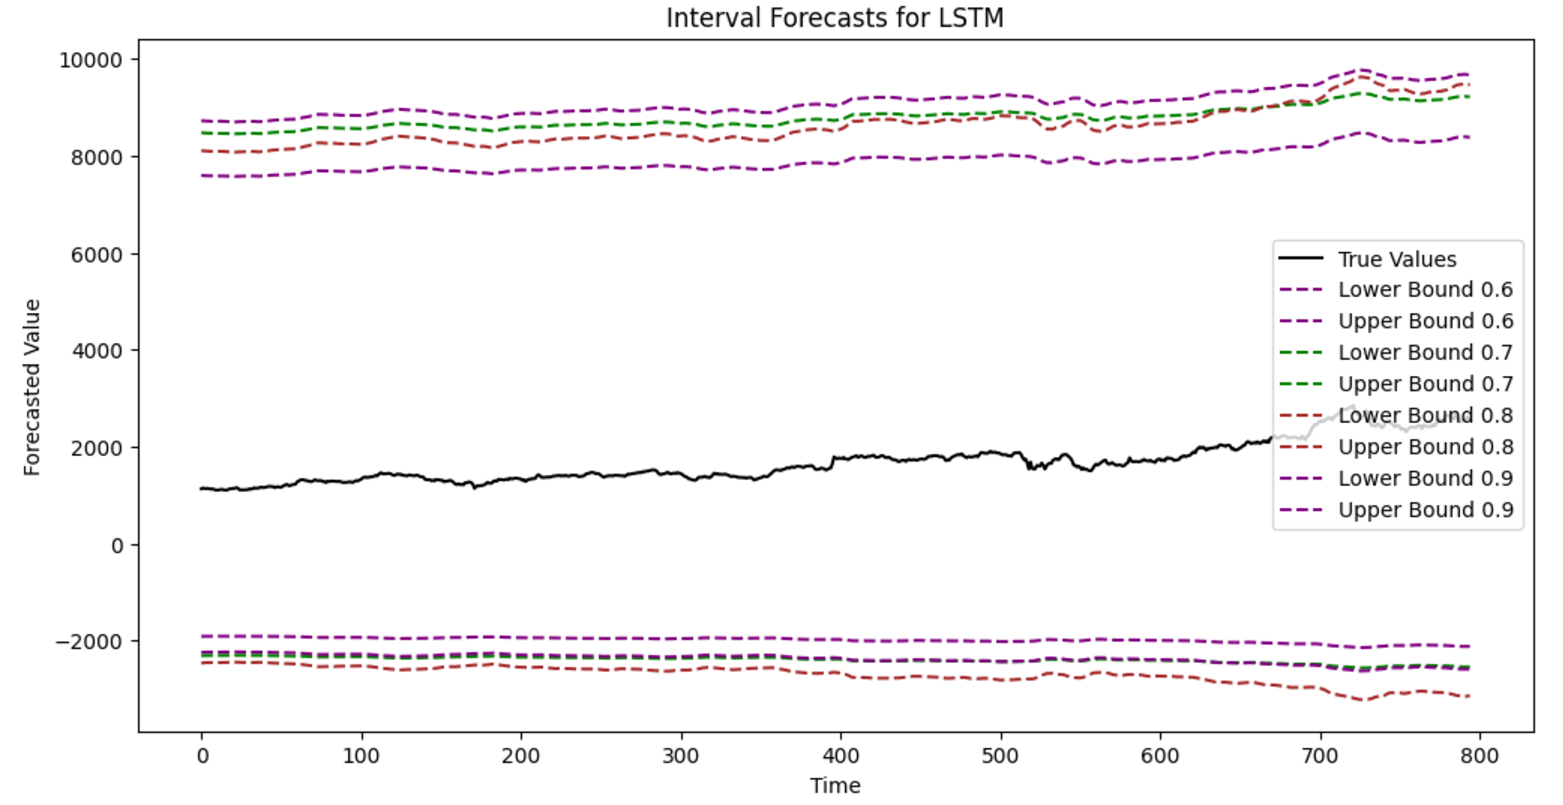
\includegraphics[width=\linewidth]{LUBE_LSTM_AsianPaints.png}
        \caption{Prediction Intervals for Asian Paints dataset obtained using Traditional LUBE method and LSTM model.}
        \label{fig:asianpaints}
    \end{minipage}
    \hfill
    \begin{minipage}[b]{0.50\linewidth}
        \centering
        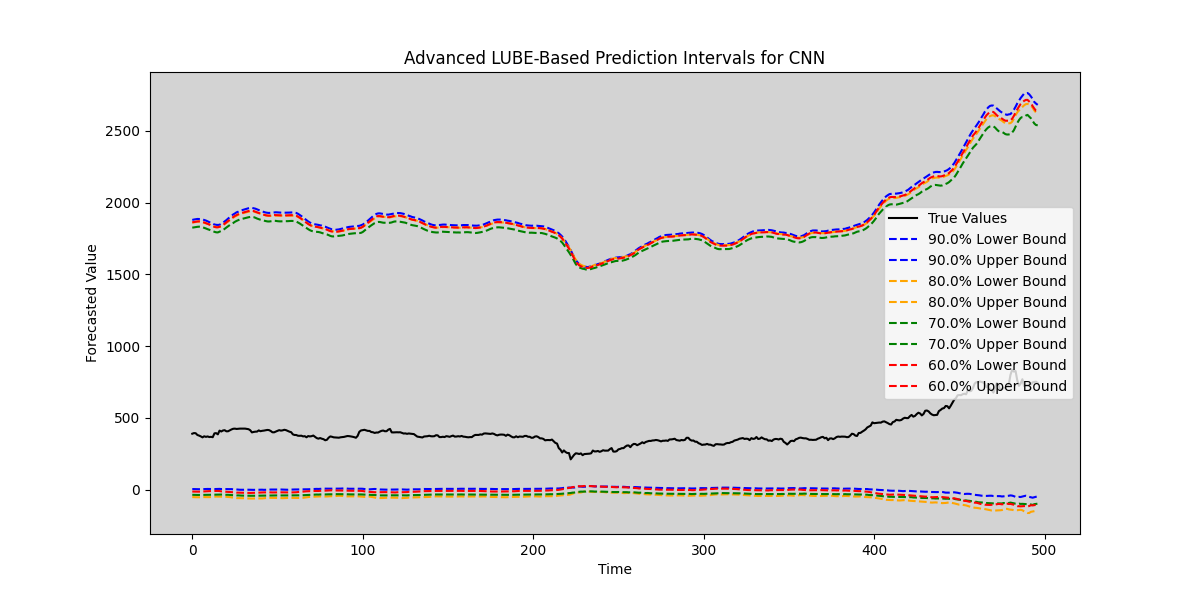
\includegraphics[width=\linewidth]{CNN_advanced_lube_plot_ADANIPORTS.png}
        \caption{Prediction Intervals for Adani Ports dataset obtained using Advanced LUBE method and CNN model.}
        \label{fig:adaniports}
    \end{minipage}
\end{figure}

\end{frame}

\begin{frame}{Graphical Analysis (Cont.)}

\begin{figure}
    \centering
    \begin{minipage}[b]{0.45\linewidth}
        \centering
        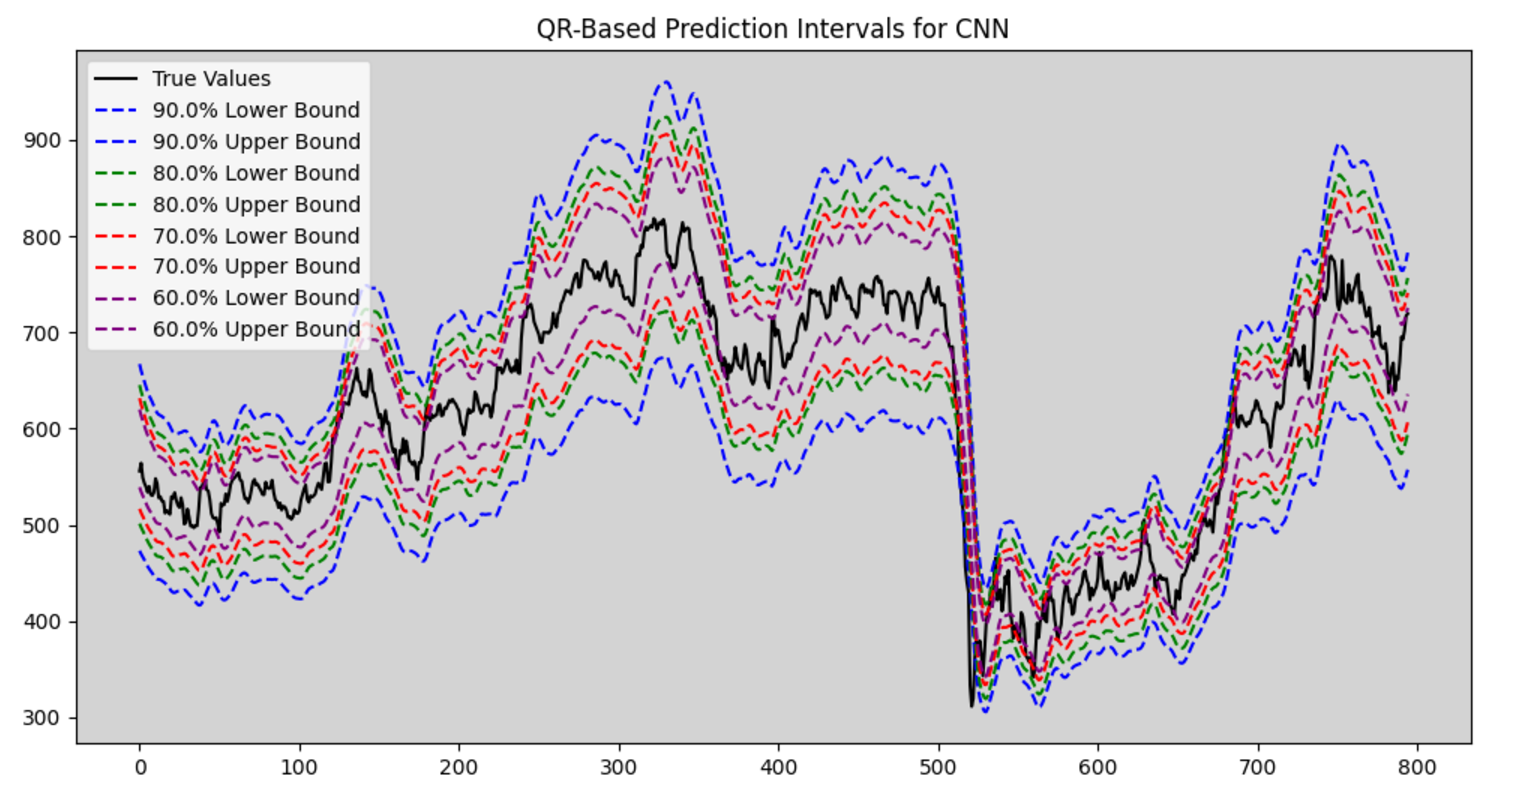
\includegraphics[width=\linewidth]{QR_CNN_AxisBank.png}
        \caption{Prediction Intervals for Axis Bank dataset obtained using QR-based method and CNN model.}
        \label{fig:asianpaints}
    \end{minipage}
    \hfill
    \begin{minipage}[b]{0.45\linewidth}
        \centering
        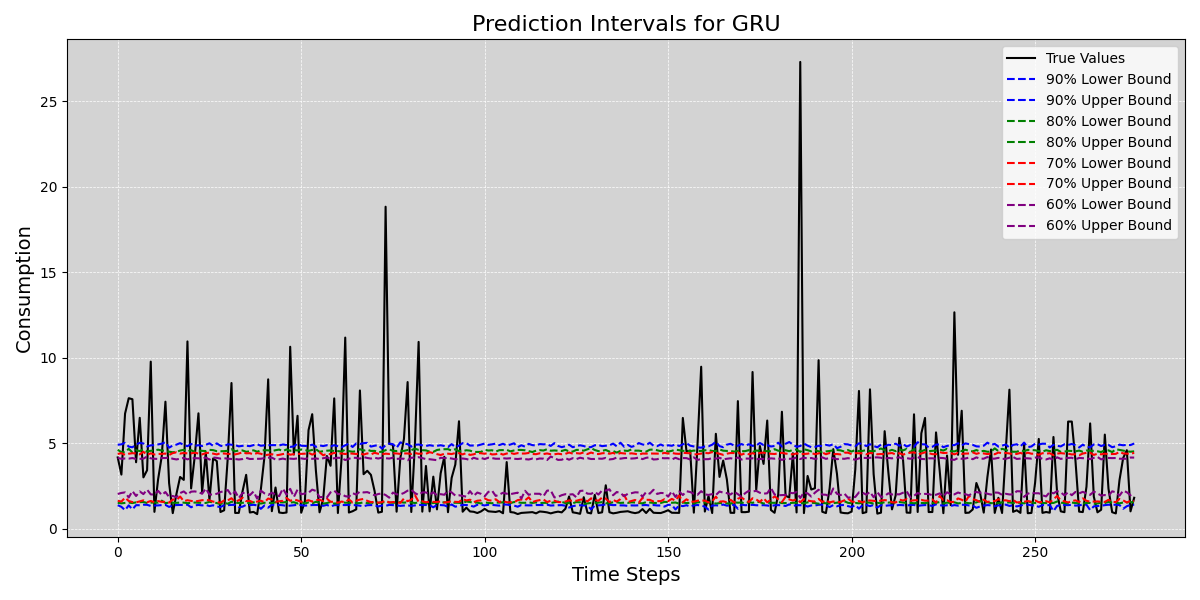
\includegraphics[width=\linewidth]{Prediction_Intervals_Styled_GRU_Electricity_Consumption.png}
        \caption{Prediction Intervals for Electricity Consumption dataset obtained using Bootstrap-based method and GRU model.}
        \label{fig:adaniports}
    \end{minipage}
\end{figure}

\end{frame}



\begin{frame}{Graphical Analysis (Cont.)}

\begin{figure}
    \centering
    \begin{minipage}[b]{0.45\linewidth}
        \centering
        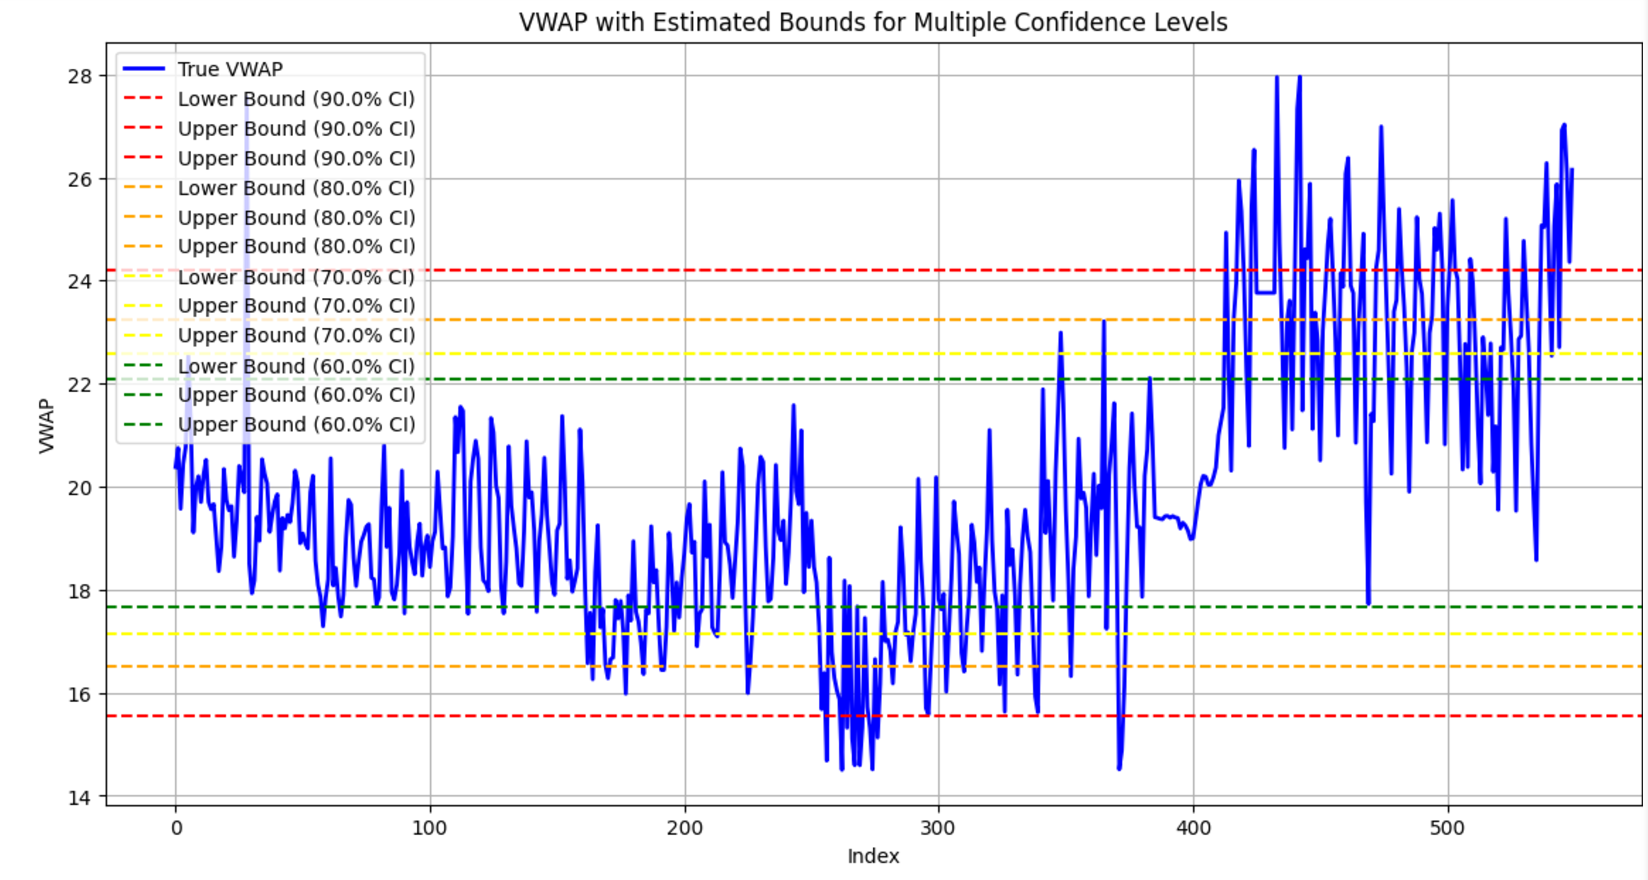
\includegraphics[width=\linewidth]{Gaussian_Web_Traffic.png}
        \caption{Prediction Intervals for Web Traffic dataset obtained using Gaussian Distribution based method.}
        \label{fig:asianpaints}
    \end{minipage}
    \hfill
    \begin{minipage}[b]{0.45\linewidth}
        \centering
        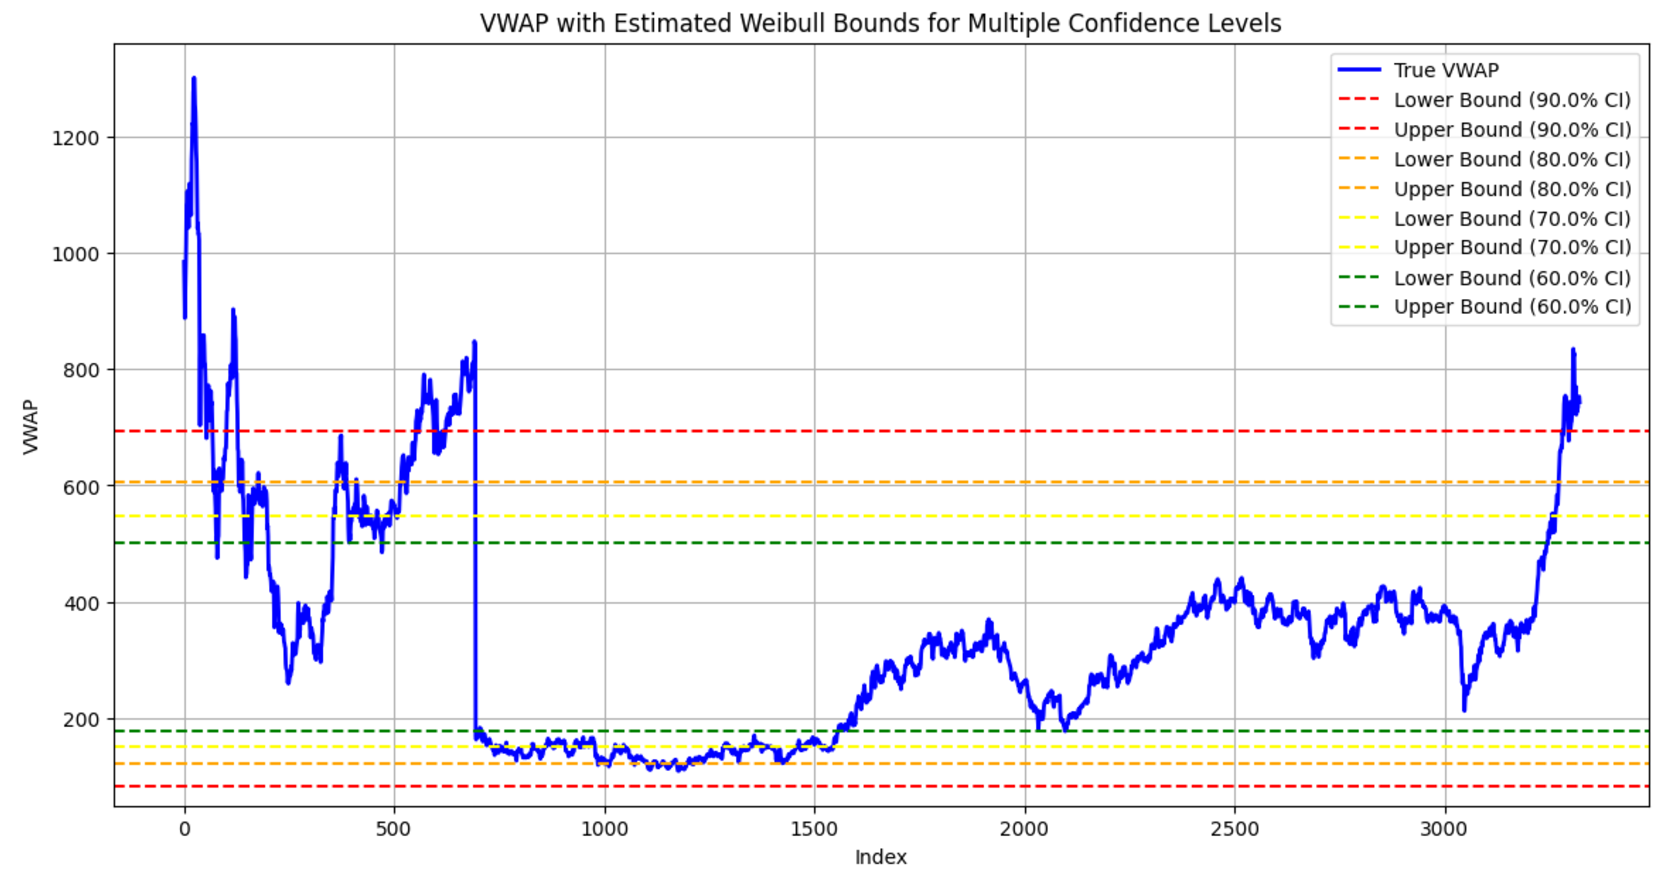
\includegraphics[width=\linewidth]{Weibull_AdaniPorts.png}
        \caption{Prediction Intervals for Adani Ports dataset obtained using Weibull Distribution based method.}
        \label{fig:adaniports}
    \end{minipage}
\end{figure}

\end{frame}
%%%%%%%%%%%%%%%%%%%%%%%%%%%%%%%%%%%%%%%%%%%%%%%%%%%%%%%%%%%%%%%%%%%%%%%%%%%%%
\begin{frame}{Graphical Analysis (Cont.)}

\begin{figure}
    \centering
    \begin{minipage}[b]{0.45\linewidth}
        \centering
        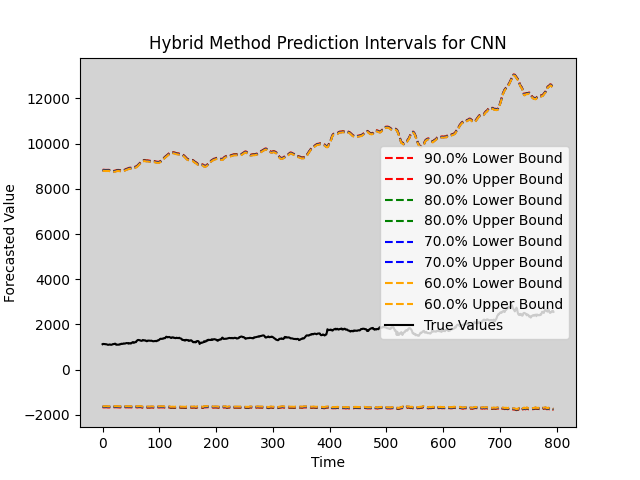
\includegraphics[width=\linewidth]{CNN_hybrid_method_plot_AsianPaint_Method2.png}
        \caption{Prediction Intervals for Asian Paints dataset obtained using LUBE-Weibull based hybrid method with CNN model.}
        \label{fig:asianpaints}
    \end{minipage}
    \hfill
    \begin{minipage}[b]{0.46\linewidth}
        \centering
        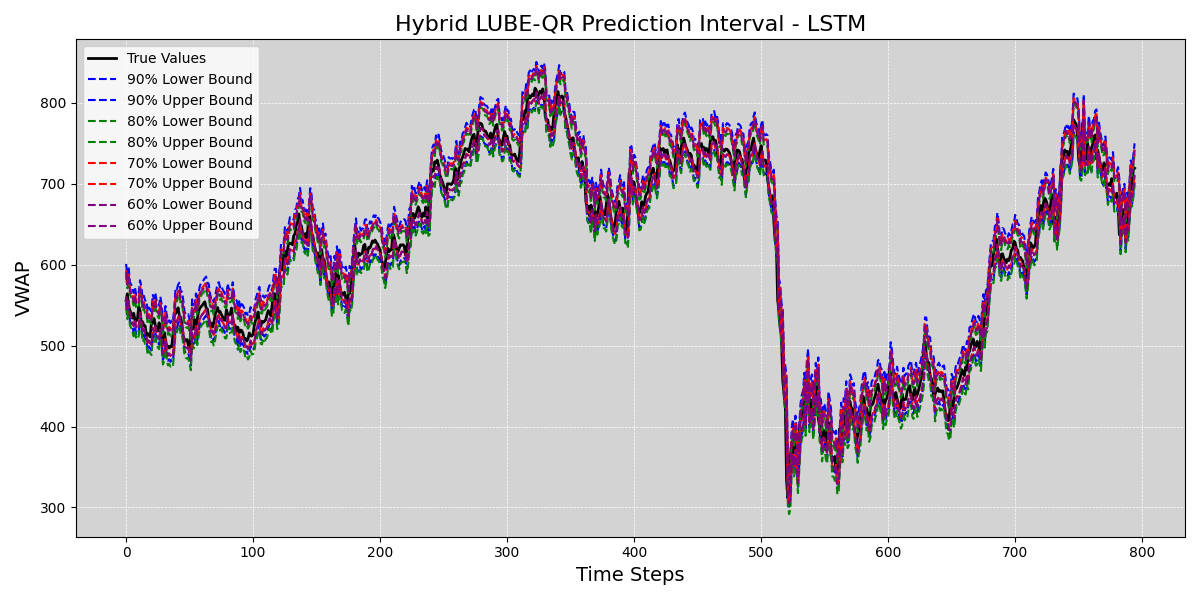
\includegraphics[width=\linewidth]{Hybrid_LUBE_QR_AllConfidence_axisbank_LSTM.png}
        \caption{Prediction Intervals for Axis Bank dataset obtained using LUBE-QR based hybrid method and LSTM model.}
        \label{fig:adaniports}
    \end{minipage}
\end{figure}

\end{frame}

\begin{frame}{Statistical Analysis}
    \centering
    \begin{minipage}[b]{0.48\linewidth}
        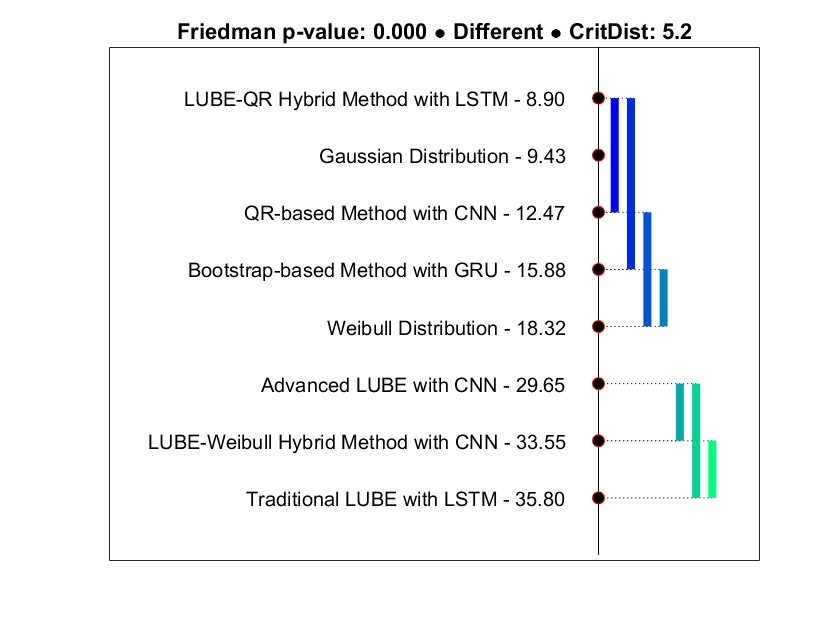
\includegraphics[width=\linewidth]{Statistical_Analysis_All_Methods_PINAW (1).jpg}
        \captionof{figure}{Friedman-Nemenyi Hypothesis Test on PINAW Metric performed on all the five datasets together.}
    \end{minipage}
    \hfill
    \begin{minipage}[b]{0.48\linewidth}
        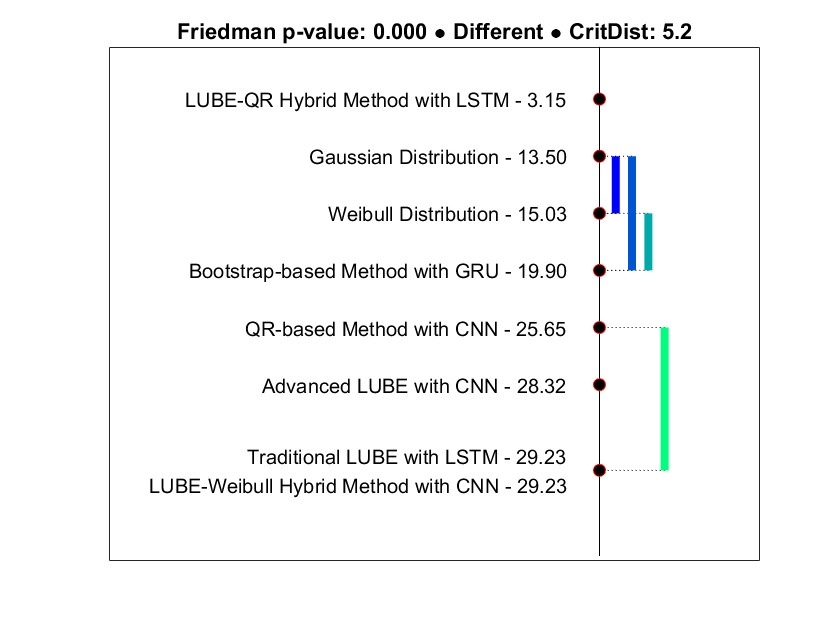
\includegraphics[width=\linewidth]{Statistical_Analysis_All_Methods_ACE (1).jpg}
        \captionof{figure}{Friedman-Nemenyi Hypothesis Test on ACE Metric performed on all the five datasets together.}
    \end{minipage}
\end{frame}


\begin{frame}{Statistical Analysis (Cont.)}
\begin{itemize}
    \item Friedman-Nemenyi hypothesis results (Figs. 18 and 19) show PINAW and ACE metric comparisons across five datasets and eight forecasting methods (each paired with its best-performing DL model).
    \item The proposed LUBE–QR based Hybrid Method is found to be statistically better than other forecasting methods assessed.
\end{itemize}
    
\end{frame}

%%%%%%%%%%%%%%%%%%%%%%%%%%%%%%%%%%%%%%%%%%%%%%%%%%%%%%%%%%%%%%%%%%%%%%%%%%
\section{Conclusion and Future Work}

%\section{Conclusion}
\begin{frame}{Conclusion}

\begin{itemize}
\item The Advanced LUBE method gave 100\% PICP values consistently across all the datasets while maintaining low PINAW and AWE Values. These results show that this method is a highly reliable method with a drawback of wider intervals (i.e conservative interval widths). 

\item Among the parametric methods, Gaussian Distribution showed promising results but it is limited by its assumption of normality and fixed width intervals, making it unsuitable for complex, non-stationary time series with dynamic patterns.
\end{itemize}
\end{frame}

\begin{frame}{Conclusion (Cont.)}
    \begin{itemize}

        \item The proposed LUBE-Weibull hybrid method is a computationally efficient alternative to computationally expensive methods. It achieved consistent results at par with Advanced LUBE method at PICP metric while being slightly worse on PINAW and AWE metric values. However because of it's efficiency, it can be a good alternative for situations that demands low computational forecasting.
        
        \item The proposed LUBE-QR hybrid method performed the best out of all the methods assessed. It achieved desirable PICP values across each dataset and confidence levels while having the least PINAW, ACE and AWE values. It was also determined to be the best method statistically by Friedman-Nemenyi Hypothesis test.
    \end{itemize}
\end{frame}


\begin{frame}{Future Work}
    \begin{itemize}
        \item Future Work may include deep diving into more hybrid methods by combining and fusing multiple existing methods with various different DL models to achieve better probabilistic forecasting results.

        \item Extend current methods to handle multiple correlated time series jointly with shared uncertainty modeling.
    \end{itemize}
\end{frame}
%%%%%%%%%%%%%%%%%%%%%%%%%%%%%%%%%%%%%%%%%%%%%%%%%%%%%%%%%%%%%%%%%%%%%%%%%%%%%%%%%%%%%%%%%%%%%%


%%%%%%%%%%%%%%%%%%%%%%%%%%%%%%%%%%%%%%%%%%%%%%%%%%%%%%%%%%%%%%%%%%%%%%%%%%%%%%%%%%%%%%%%%


%%%%%%%%%%%%%%%%%%%%%%%%%%%%%%%%%%%%%%%%%%%%%%%%%%%%%%%%%%%%%%%%%%%%%%
\section{}
\begin{frame}{References} 
\footnotesize
\begin{thebibliography}{99}
\bibliographystyle{plain}
\bibliography{new}
\nocite{*}

\end{thebibliography}
\end{frame}
%%%%%%%%%%%%%%%%%%%%%%%%%%%%%%%%%%%%%%%%%%%%
\section{}
\begin{frame}{}
\LARGE
\centerline{Thank You}
    
\end{frame}

%%%%%%%%%%%%%%%%%%%%%%%%%%%%%%%%%%%%%%%%%%%%%%%%%%%%%%%%%%%%%%%%%%%%%%%%%%%%

%%%%%%%%%%%%%%%%%%%%%%%%%%%%%%%%%%%%%%%%%%%%%%%%%%%%

\end{document}
    
